\documentclass[a4paper]{article}
\usepackage[dutch]{babel}
\usepackage{float}
\usepackage{graphicx}
\usepackage{verbatim}
\setlength{\parindent}{0ex}
\setlength{\parskip}{1ex}

\begin{document}

\section*{Spoorhekcodering}
\flushright
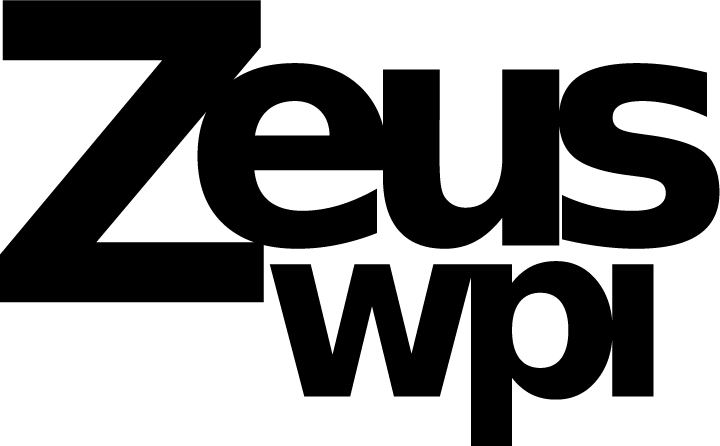
\includegraphics[width=3em]{../logo-new.png}
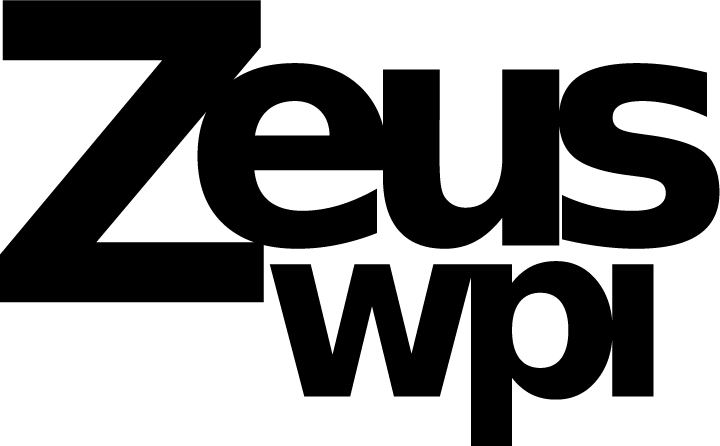
\includegraphics[width=3em]{../logo-new.png}
\flushleft

Bij spoorhekcodering (of zigzagcodering) worden de letters van een gegeven tekst
eerst diagonaal naar beneden uitgeschreven op opeenvolgende "sporen" van een
denkbeeldig hek. Nadat het onderste spoor bereikt wordt, gaat het uitschrijven
van de letters diagonaal naar boven verder. De tekst wordt opnieuw diagonaal
naar beneden uitgeschreven, van zodra het bovenste spoor bereikt wordt. Deze
procedure herhaalt zich totdat alle letters van de tekst uitgeschreven zijn. Als
we bijvoorbeeld op vier sporen de tekst "And now for something completely
different." uitschrijven, dan krijgen we

\begin{verbatim}
A#####w#####s#####i#####m#####l#####f#####.
#n###o# ### #o###h#n###o#p###e#y###f#e###t#
##d#n###f#r###m#t###g#c###l#t### #i###r#n##
### #####o#####e##### #####e#####d#####e###
\end{verbatim}

De gecodeerde tekst wordt gevormd door de letters per spoor van links naar
rechts achter elkaar te zetten, en dit vanaf het bovenste spoor tot het onderste
spoor. De gecodeerde boodschap voor de bovenstaande voorbeeldtekst leest dan als
"Awsimlf.no  ohnopeyfetdnfrmtgclt irn oe ede".

\subsection*{Input}

Op de eerste lijn van de input vind u zoals steeds het aantal gevallen. Per
geval volgen er dan twee lijnen. De eerste van deze twee lijnen houd de
opdracht. Deze bestaat uit 2 woorden, waarvan het eerste telkens \texttt{encode}
of \texttt{decode} zal zijn. Het tweede woord is een strikt positief geheel
getal dat het aantal sporen oplegd. Op de tweede lijn van het geval volgt dan de
te (de)coderen boodschap.

\subsubsection*{Voorbeeldinput}

\verbatiminput{voorbeeld.invoer}

\subsection*{Output}

Per geval verwachten we \'e\'en lijn output, zijnde de ge(de)codeerde boodschap.

\subsubsection*{Voorbeeldoutput}

\verbatiminput{voorbeeld.uitvoer}

\end{document}
